\documentclass[11pt]{beamer}
\usepackage{booktabs}
\usepackage{array}
\usepackage{eulervm}
\usepackage{tcolorbox}
\usepackage[export]{adjustbox}
\usepackage{tikz}
\usepackage{minted}
\usemintedstyle{gruvbox-light}
\newcommand{\R}[1]{\mintinline[escapeinside=||]{r}{#1}}

\newcommand{\sgap}{\vspace{0.5em}}
\newcommand{\bgap}{\vspace{0.8em}}

\newcommand\Wider[2][3em]{%
\makebox[\linewidth][c]{%
  \begin{minipage}{\dimexpr\textwidth+#1\relax}
  \raggedright#2
  \end{minipage}%
  }%
}

% Fonts --------------------------------------------------------------------------

\usepackage[scaled]{helvet}
\usepackage[T1]{fontenc}
\usepackage[scale=0.95]{inconsolata}

% If using XeLaTeX:
% \usepackage{fontspec}
% \setmonofont[Path=./fonts/,Scale=0.9]{JetBrainsMono.ttf}
% \setmainfont[Path=./fonts/]{KingsBureauGrot-FiveOne.ttf}
% \setsansfont[Path=./fonts/]{KingsCaslon.ttf}
% \setbeamerfont{title page}{family=\rmfamily}
% \setbeamerfont{frametitle}{family=\rmfamily}

% References ------------------------------------------------------------------

\usepackage[%
  backend     = bibtex,
  style       = numeric,
  sorting     = ynt,
  sortcites   = true,
  autocite    = superscript
]{biblatex}

\addbibresource{references.bib}

% tcolorbox -------------------------------------------------------------------

\newtcolorbox{cbox}[3][]
{
  colframe = #2!5,
  colback  = #2!5,
  coltitle = #2!50!black,  
  colbacktitle = #2!5,
  lefttitle = 1mm,
  toptitle = 2mm,
  bottomtitle = 0mm,
  colupper = #2!50!black,  
  title    = {#3},
  fonttitle = \bfseries\large,
  #1,
  arc=0.5mm,
  left=2.5mm,
  before upper={\setbeamercolor{item}{fg=#2!50!black}},
  after upper={\setbeamercolor{item}{fg=#2!50!black}}
}

\makeatletter
\def\beamer@origitem{%
  \@inmatherr\item\@ifnextchar[\@item{\@noitemargtrue\@item[\@itemlabel]%
  \csname beamer@thcfg@\beameritemnestingprefix item\endcsname% Insert colour in \beamer@thc@fg
  \ifx\beamer@thc@fg\@empty\relax\else\color{\beamer@thc@fg}\fi% Execute colour
  }}
\makeatother

\usepackage{graphicx}
\newcommand*{\img}[1]{%
    \raisebox{-.3\baselineskip}{%
        \includegraphics[
        height=\baselineskip,
        width=\baselineskip,
        keepaspectratio,
        ]{#1}%
    }%
}

\newcommand*{\timg}[2]{%
	\raisebox{-.5#1}{%
		\includegraphics[
			width=#1
		]{#2}%
    }%
}

\title[The pmsims package for R]{
    A simulation approach to calculating minimum sample sizes for prediction
    modelling
}
\subtitle{The pmsims package for R}
\date{29$^{\text{th}}$ August 2023}
\author[Biostatistics \& Health Informatics, KCL]{%
	Ewan Carr, Gordon Forbes, Diana Shamsutdinova, Daniel Stahl,
	and Felix Zimmer}
\institute[]{Department of Biostatistics \& Health Informatics\\ King's College London}
\titlegraphic{
\includegraphics[height=1.5cm]{figures/kcl.png}}
\setbeamertemplate{navigation symbols}{}
\setbeamertemplate{footline}[frame number]

% Theme
\definecolor{KCLpurple}{RGB}{80, 20, 145}
\definecolor{KCLred}{RGB}{226, 35, 26}
\definecolor{KCLhotpink}{RGB}{200, 50, 150}
\definecolor{KCLpurple}{RGB}{80, 20, 145}
\definecolor{KCLseablue}{RGB}{0, 90, 210}
\definecolor{KCLtealblue}{RGB}{0, 154, 166}
\definecolor{KCLpeagreen}{RGB}{0, 181, 136}
\definecolor{KCLpantone}{RGB}{0, 35, 149}
\usecolortheme[named=KCLseablue]{structure}
\setbeamercolor{alerted text}{fg=KCLhotpink}

\setbeamertemplate{itemize items}[circle]
\setbeamertemplate{enumerate items}[default]

\newenvironment{itemize*}%
{\begin{itemize}%
		\setlength{\itemsep}{100pt}%
		\setlength{\parskip}{0pt}}%
		{\end{itemize}}

\begin{document}

\maketitle

\section{Introduction}

\begin{frame}[c]{30-second version}
	\Large
	\begin{enumerate}
		\setlength{\itemsep}{12pt}

		\item Most prediction models use small samples.

		\item Small samples cause overfitting and imprecise estimates.

		\item Existing tools can estimate minimum samples for continuous,
		      binary, and survival outcomes.

		\item Nothing exists for other models or data types.

	\end{enumerate}

	\sgap

	\begin{cbox}{KCLtealblue}{}
		We're developing a simulation-based approach that works with any
		outcome or method.
	\end{cbox}
	\vspace{-1em}
\end{frame}

\begin{frame}[c]
	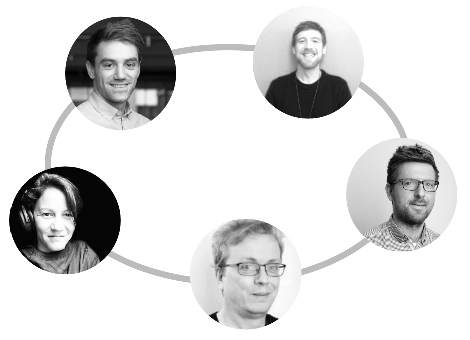
\includegraphics[width=\textwidth]{figures/group_photos.pdf}
\end{frame}

\begin{frame}[t]{This talk}
    \sgap
	\Large
	\begin{enumerate}
		\item Background
		      \begin{itemize}
			      \item What's the problem we're trying to solve?
			      \item What solutions currently exist?
		      \end{itemize}
		\item Our simulation-based approach
		      \begin{itemize}
			      \item Workflow and user interface
			      \item How it compares to other packages
		      \end{itemize}
		\item Demonstration
		\item Development status and next steps
	\end{enumerate}

    \onslide<2->
    \normalsize
	\vspace{6mm}
	\begin{cbox}{KCLtealblue}{}
		\centering
		
\includegraphics[width=4em,valign=c]{figures/construction-site.pdf}
		\hspace{2em} {\large Under construction; feedback welcome.}
	\end{cbox}

\end{frame}

\section{Background}

\begin{frame}[t]{What's the problem?}

	% Say: Prediction models can inform treatment decisions, facilitate
	% screening, and enable stratified care.

	Hundreds of prediction models are developed each year. Most have
	inadequate samples.

	\begin{cbox}{KCLseablue}{}
		\large
		\begin{itemize}
			\item Insufficient sample sizes was the most common cause of bias
			      in 731 models for COVID-19.\autocite{wynants2020}
			\item Inadequate samples were found in: \vspace{0.5em}
		\end{itemize}
		\begin{tabular}{lp{.8\textwidth}}
			{\Huge \alert{67\%}} & models for COVID-19\autocite{wynants2020}                      \\[0.5em]
			{\Huge \alert{56\%}} & models using supervised machine learning\autocite{navarro2021} \\[0.5em]
			{\Huge \alert{73\%}} & models in psychiatry\autocite{meehan2022}                      \\[0.3em]
		\end{tabular}
		\begin{itemize}
			\item Just \alert{8\%} of machine learning models in oncology
			      reported a sample size justification\autocite{dhiman2022}.
		\end{itemize}
	\end{cbox}
\end{frame}

\begin{frame}[t]{Inadequate samples = research waste}

	\begin{itemize}
		\item Inadequate samples lead to overfitting and inaccurate estimates
		      of model parameters.

		      % Overfitting is where the model captures idiosyncrasies
		      % of the development sample, producing inflated estimates of predictive
		      % performance that cannot be replicated in the target population.

		\item This may generate inappropriate decisions about patient care or
		      lead to models not being implemented into clinical practice.

		\item Data collection can be invasive and inconvenient and diverts
		      resources from other activities that benefit patients.

	\end{itemize}

	\begin{cbox}{KCLpurple}{}
		\large
		Ensuring sample sizes are sufficient \textbf{before model development}
		would improve patient outcomes by avoiding models developed with
		inadequate samples and reducing participant burden.
	\end{cbox}

\end{frame}

\begin{frame}[t]{What tools exist?}

	\centering
	\begin{columns}
		\begin{column}[c]{0.6\textwidth}
			\centering
			Most studies ignore sample size.
			\bgap%

			Or use rules of thumb (e.g., 10 events per variable) that have no
			rationale in prediction modelling\autocite{vansmeden2016}.
		\end{column}
		\begin{column}[c]{0.4\textwidth}
			
\includegraphics[width=\textwidth]{figures/bury-head.png}%
		\end{column}
	\end{columns}

	% This rule of thumb has been shown to have no rationale, especially
	% in prediction model research, as its evidence base is mainly informed by
	% simulation studies that investigate the performance of estimating
	% covariate-outcome relationships.
	% https://bmcmedresmethodol.biomedcentral.com/articles/10.1186/s12874-023-02008-1
    \bgap

	\begin{columns}
		\begin{column}[c]{0.5\textwidth}
			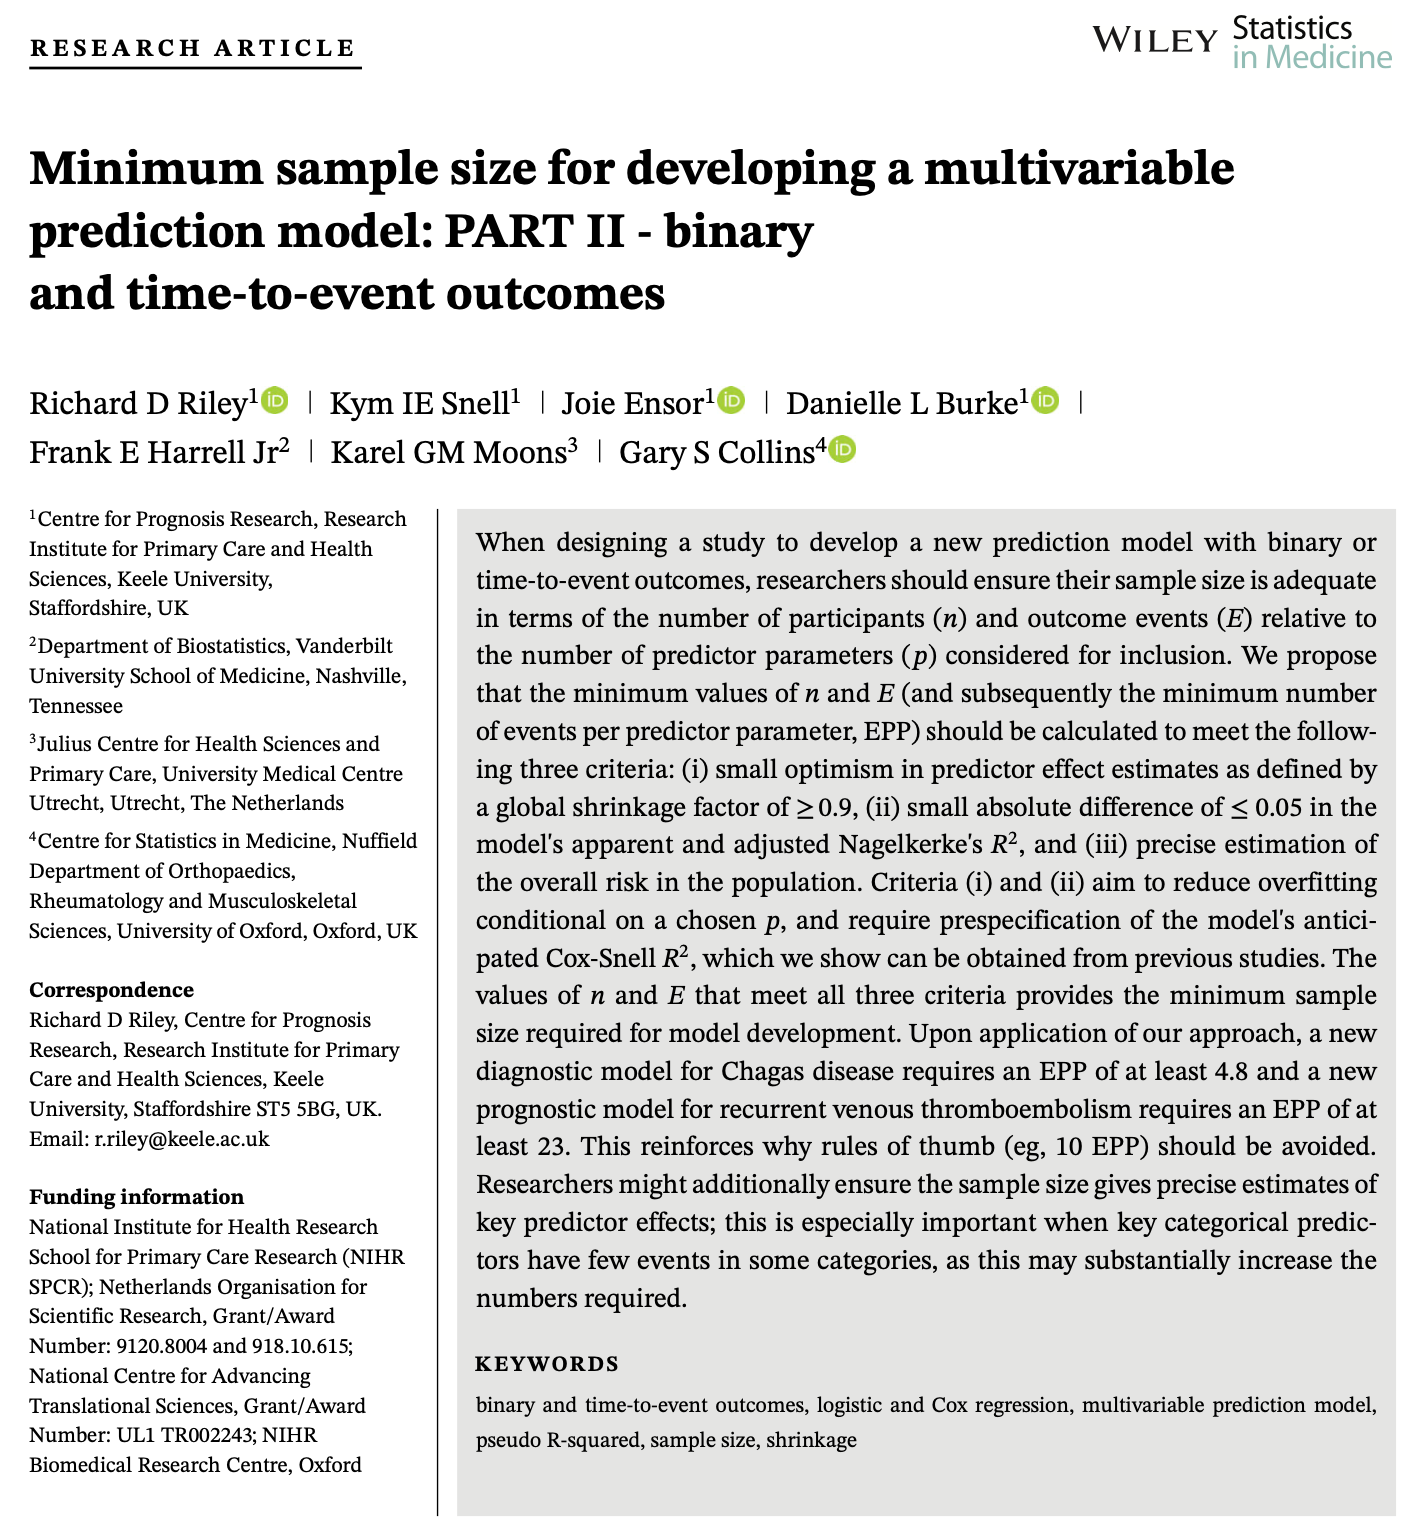
\includegraphics[width=\textwidth]{figures/riley2.png}%
		\end{column}
		\begin{column}[c]{0.5\textwidth}
            In 2018, Riley et al.\ released \alert{pmsampsize} for R and Stata.
		\end{column}
	\end{columns}

\end{frame}

\begin{frame}[c]{We \img{figures/heart.png} pmsampsize, but\ldots}
	\large

	pmsampsize provides methods for continuous, binary, and survival
	outcomes. But we increasingly need to estimate minimum samples for:

	\begin{cbox}{KCLtealblue}{Other models}
		\begin{itemize}
			\item Regularised regression (e.g., LASSO, elastic net)
			\item Machine learning algorithms (e.g., random forests, gradient
			      boosting)
		\end{itemize}
	\end{cbox}

	\begin{cbox}{KCLhotpink}{Other types of data}{}
		\begin{itemize}
			\item Longitudinal and repeated measures
			\item Clustered data
		\end{itemize}
	\end{cbox}

	We're creating a simulation-based framework to estimate sample sizes for
	prediction.

\end{frame}

\begin{frame}[t]{The \alert{pmsims} package for R}

	Key features:

	\begin{itemize}
		\item Able to estimate minimum sample sizes for \alert{any model or
		      data type};
		\item Provides defaults for common model and data types;
		\item Efficient estimation.
	\end{itemize}

	This last point is key:\ most machine learning approaches are too
	computationally demanding for conventional simulation approaches.

\end{frame}

\begin{frame}[t]{Our approach}

	\begin{cbox}{KCLpeagreen}{Setting}
		\begin{enumerate}
			\setlength{\itemsep}{7pt}
			\item A study population represented by outcome-related individual
			      characteristics (i.e., candidate predictors).
			\item A chosen statistical or machine learning model.
			\item Expected achievable performance (e.g., $R^2$, AUC) without
			      sample size constraints, $P^{*}$.
			\item Minimum acceptable performance of the model, $P^{OK}$.
		\end{enumerate}
	\end{cbox}

	\onslide<2>
	\bgap
	\centering
	
\includegraphics[height=3.6em]{figures/target.pdf}
	\hspace{0.7em}
	\large
	\parbox[b]{0.8\textwidth}{ \raggedright \textcolor{KCLpantone}{ Find the
	    minimum sample that ensures test performance of $P^{OK}$ with
	    probability of 80\%, given the population, predictors, and $P^{*}$. }
	    }

	% i.e., drawing a random sample of size $n$ will result in a model with
	% performance $>P^{OK}$ in more than 80\% of cases.

\end{frame}

\begin{frame}{How does it work?}

	\begin{columns}[T]
		\begin{column}{0.4\textwidth}
			\centering
			\includegraphics<+>[width=0.85\textwidth]{figures/workflow-b.pdf}%
			\includegraphics<+>[width=0.85\textwidth]{figures/workflow-c.pdf}%
			\includegraphics<+>[width=0.85\textwidth]{figures/workflow-d.pdf}%
			\includegraphics<+>[width=0.85\textwidth]{figures/workflow-e.pdf}%
		\end{column}
		\begin{column}{0.7\textwidth}
			\only<1>{
				\vspace{1em}
				The user specifies:
				\begin{enumerate}
					\item The candidate predictors (number, type)
					\item The chosen statistical model
					\item The expected large sample performance ($P^{*}$)
					\item The minimum acceptable performance ($P^{OK}$)
				\end{enumerate}
			}%
			\only<2>{
				\vspace{6em}
				Based on their input, we set:
				\begin{enumerate}
					\item A data generating function
					\item A model function
					\item A metric function
				\end{enumerate}
			}%
			\only<3>{
				\vspace{11em}
				We then tune the data generating model, so the large sample
				performance is $P^{*}$.
			}
		\end{column}
	\end{columns}

\end{frame}

\begin{frame}[t]{Performing the search}
	\tikz[overlay, remember picture]
	\node[%
		anchor=north east,
		yshift=0.2cm,
		xshift=-0.5cm]at (current page.north east) {
		\includegraphics[width=0.3\textwidth]{figures/tortoise.png}%
	};

	\vspace{-0.5em}
	An exhaustive grid search would be too slow.
	\Wider{%
		\vspace{2em}
		\begin{cbox}{KCLpurple}{Surrogate modelling with mlpwr}
			% Surrogate modeling aims to approximate a relationship that is costly to
			% investigate with a cheaper function.

			\begin{itemize}
				\item Approximates relationship between sample size and
				      $P^{OK}$ using Guassian process regression.
				\item Also referred to as `learning curve
				      fitting'\autocite{figueroa2012, dayimu2023}.
				\item Uses the mlpwr R package by Zimmer and
				      Debelak\autocite{zimmer2022}.
			\end{itemize}
		\end{cbox}

		\vspace{0.3em}
		\centering
		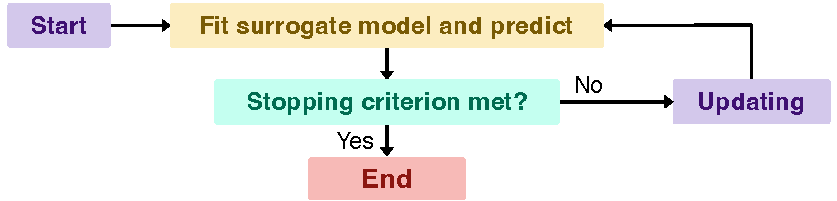
\includegraphics[width=\textwidth]{figures/surrogate_algorithm.pdf}%
	}
\end{frame}

\begin{frame}[c]{Surrogate modelling}

	\includegraphics<+>[width=\textwidth]{figures/surrogate-1.pdf}%
	\includegraphics<+>[width=\textwidth]{figures/surrogate-3.pdf}%
	\includegraphics<+>[width=\textwidth]{figures/surrogate-4.pdf}%
	\includegraphics<+>[width=\textwidth]{figures/surrogate-5.pdf}%
	\includegraphics<+>[width=\textwidth]{figures/surrogate-6.pdf}%
	\includegraphics<+>[width=\textwidth]{figures/surrogate-7.pdf}%
	\includegraphics<+>[width=\textwidth]{figures/surrogate-8.pdf}%

\end{frame}

\begin{frame}[t]{How do we assess performance?}

	\Wider{
		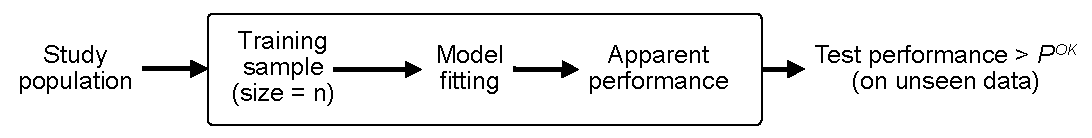
\includegraphics[width=\textwidth]{figures/performance_flow.pdf}%

		We identify the minimum sample that meets \underline{two} criteria:

		\begin{cbox}{KCLpeagreen}{}
			{\large
				\textbf{1.\ Discrimination} \\

				Within 0.1 of the achievable large sample discrimination,
				$P^*$. }

			\bgap

			The threshold and metric can be chosen by users.
		\end{cbox}

		\begin{cbox}{KCLpantone}{}
			{\large
				\textbf{2.\ Calibration} \\

				A calibration slope of 0.9 to 1.1.}
		\end{cbox}

		But we're open to suggestions. }

\end{frame}

\begin{frame}[t]{Two approaches to estimating minimum samples}

	\footnotesize
	\Wider[5em]{
		\begin{tabular}{lp{0.4\textwidth}p{0.4\textwidth}}
			                                   & {\Large \textcolor{KCLpurple}{pmsims}}                                                                 & {\Large \textcolor{KCLhotpink}{pmsampsize}}        \\
			Target?                            & Minimum development sample that ensures expected apparent and test performances are sufficiently close &
			Minimum development sample that ensures test performance of $P^{OK}$ with 80\% probability                                                                                                       \\[14mm]
			How?                               & {\large \textcolor{KCLpurple}{Simulate}}                                                               & {\large \textcolor{KCLhotpink}{Uniform shrinkage}} \\
			                                   &
			\begin{minipage}[t]{0.4\textwidth}
				\begin{itemize}
					\item Tune data generator to an expected achievable
					      performance.
					\item Sample training data of different sizes, compute
					      performance metrics. Using mlpwr find n at which 0.2
					      quantile of test performances achieves Pok.
					\item NB pmsims handles calibration slope as a performance
					      measure, which is the same as uniform shrinkage, as
					      slope is defined as minimizing the error between
					      $y^{test}$ and ($\alpha + slope \times
					      \hat{y}^{test}$).
				\end{itemize}
			\end{minipage} &
			\begin{minipage}[t]{0.4\textwidth}
				\begin{itemize}
					\item Consider GLM models, where estimates depend on a
					      linear predictor, $x^{T}\hat{\beta}$, with
					      $\hat{\beta}-$ OLS/ML estimates from the training
					      sample.
					\item Using $s \cdot x^{T}\hat{\beta}$, instead of
					      $x^{T}\hat{\beta}$ may prevent overfitting and
					      perform better on unseen cases.
				\end{itemize}
			\end{minipage}
		\end{tabular}
	}

	Diana slide 2 - how our criteria compare to pmsampsize

\end{frame}

\begin{frame}[t]
	\footnotesize
	\Wider[4.5em]{
		\begin{tabular}{@{}p{0.5\textwidth}@{}p{0.5\textwidth}}
			{\Large pmsims}                     & {\Large pmsampsize} \\
			\begin{minipage}[t]{0.45\textwidth}
				\begin{itemize}
					\item Targets absolute performance
					\item Flexible
					      % Machine learning, multilevel models, etc.
					      % heteroscedasticity and multicollinearity in the data
					\item Does not aim to prevent overfitting per se
					\item Targets test performance*
					\item Adjusts recommendations for test performance
					      variance**
				\end{itemize}
				However:\
				\begin{itemize}
					\item Computationally demanding
					\item User must specify data/model for complex designs
					\item Simulation variability
				\end{itemize}
			\end{minipage} &
			\begin{minipage}[t]{0.45\textwidth}
				\begin{itemize}
					\item Fast, closed-form solutions
					\item Ensures sufficient training sample to prevent
					      overfitting
				\end{itemize}
				However:\
				\begin{itemize}
					\item Closed-form only for some
					      models\autocite{riley2021}.
					\item Does not adjust predictions to the variance of the
					      test performance\autocite{vanhouwelingen1990a}.
					\item As only one training sample will be available to the
					      model developers, actual performance once deployed
					      may be much lower**.
				\end{itemize}
			\end{minipage}
		\end{tabular}
	}

\end{frame}

\begin{frame}[t]{}
	\Wider{
		Compared to pmsampsize, we expect our approach will require:

		\begin{itemize}
			\item Lower N for machine learning models:\
			      \begin{itemize}
				      \item Tend to overfit but may still produce high test
				            performance.
				      \item Targeting shrinkage requires $\uparrow$ N compared
				            to targeting test performance
			      \end{itemize}
			\item Higher N for noisy data and models with high variance:\
			      \begin{itemize}
				      \item 0.2 quantile of test performance will
				            be lower than mean, requiring larger N
			      \end{itemize}
		\end{itemize}

		\vspace{5em}
		\centering
		Diana figure here.
	}

\end{frame}

\begin{frame}[c,fragile]{The user interface}

	\vspace{1em}
	\centering
	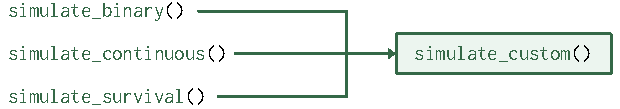
\includegraphics[width=0.9\textwidth]{figures/interfaces.pdf}%
	\vspace{-1.5em}

	\begin{columns}
		\begin{column}[t]{0.55\textwidth}
			\begin{cbox}{gray}{}
				\begin{minted}[autogobble,fontsize=\small]{r}
simulate_continuous <- 
  function(
    signal_parameters = 30,
    noise_parameters = 0,
    min_sample_size = 300,
    max_sample_size = 10000,
    large_discrimination = 0.7,
    minimum_threshold = 0.1,
    model = "lm",
    metric = "r2",
    ...
  ) 
            \end{minted}
			\end{cbox}
		\end{column}
		\begin{column}[t]{0.55\textwidth}
			\begin{cbox}{gray}{}
				\begin{minted}[autogobble,fontsize=\small]{r}
simulate_binary <- 
  function(
    signal_parameters = 30,
    noise_parameters = 0,
    baseline_prob = 0.1,
    min_sample_size = 300,
    max_sample_size = 10000,
    large_discrimination = 0.8,
    minimum_threshold = 0.1,
    metric = "auc",
    model = "glm",
    ...
  )
            \end{minted}
			\end{cbox}
		\end{column}
	\end{columns}

\end{frame}

\begin{frame}[b,fragile]{Example 1:\ Binary outcome, logistic regression}
	\Wider{
		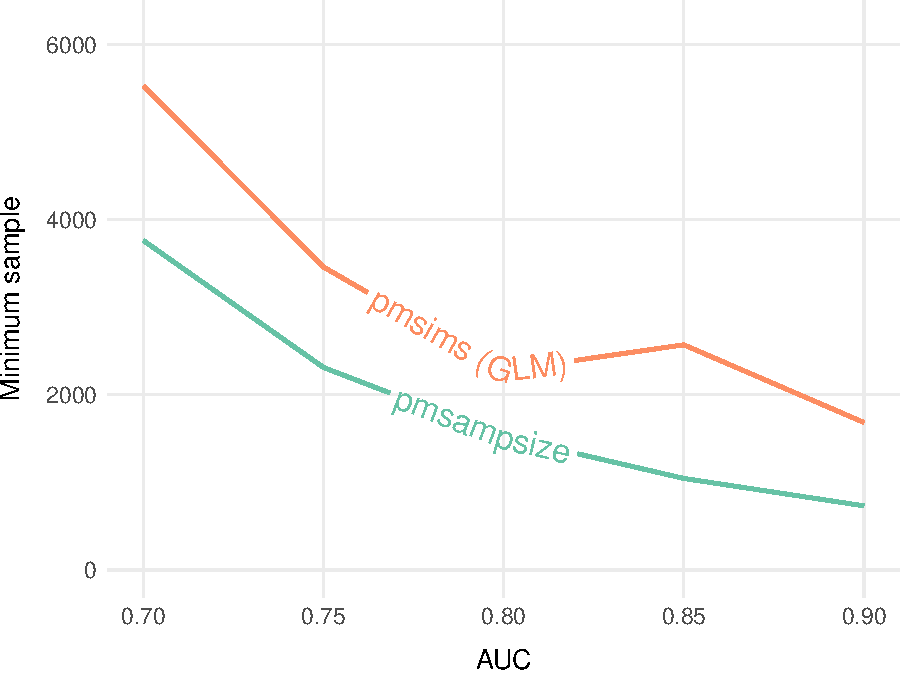
\includegraphics[width=0.9\textwidth]{figures/demo1.pdf}%
	}

	\tikz[overlay, remember picture]
	\node[anchor=north east, yshift=-0.9cm] at (current page.north east) {
		\begin{cbox}[width=4.8cm]{gray}{}%
			\begin{minted}[autogobble,fontsize=\scriptsize]{r}
simulate_binary(
  signal_parameters = 20,
  baseline_prob = 0.1,
  min_sample_size = 500,
  max_sample_size = 15000,
  large_discrimination = ...,
  minimum_threshold = 0.1,
  metric = "auc",
  model = "glm",
)
            \end{minted}
		\end{cbox}
	}2

\end{frame}

\begin{frame}[b,fragile]{Example 2:\ Binary outcome, LASSO regression}

	\Wider{
		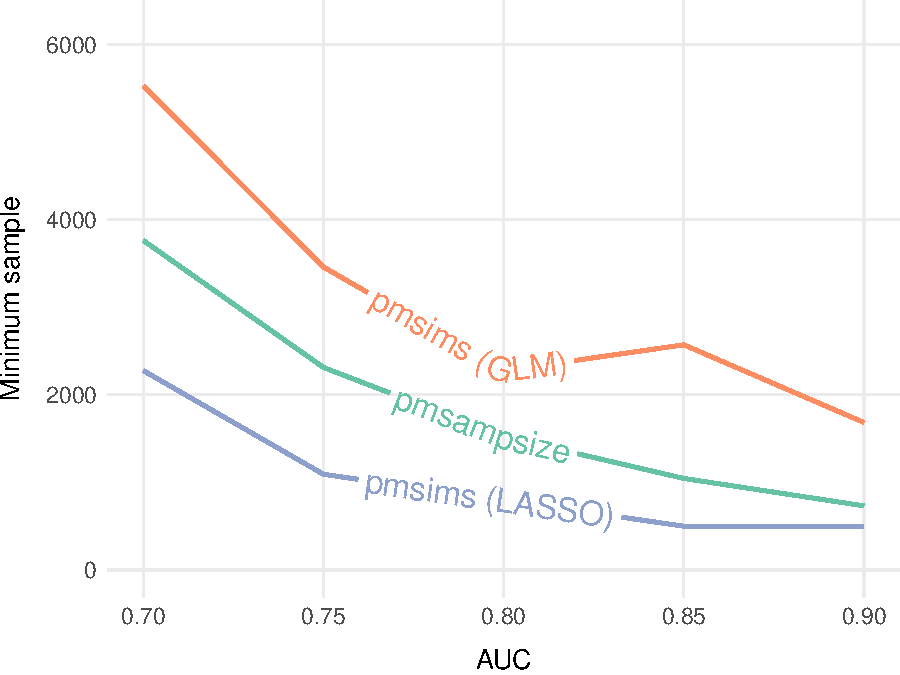
\includegraphics[width=0.9\textwidth]{figures/demo2.pdf}%
	}

	\tikz[overlay, remember picture]
	\node[anchor=north east, yshift=-0.9cm] at (current page.north east) {
		\begin{cbox}[width=4.8cm]{gray}{}%
			\begin{minted}[%
                highlightlines=9,
                autogobble,
                fontsize=\scriptsize]{r}
simulate_binary(
  signal_parameters = 20,
  baseline_prob = 0.1,
  min_sample_size = 500,
  max_sample_size = 15000,
  large_discrimination = ...,
  minimum_threshold = 0.1,
  metric = "auc",
  model = "lasso",
)
            \end{minted}
		\end{cbox}
	};

\end{frame}

\begin{frame}[c,fragile]{Example 3:\ Custom model function}

	What if a model hasn't been implemented?        \vspace{-0.5em}%%

	\begin{columns}
		\begin{column}[T]{0.5\textwidth}
			\begin{cbox}{gray}{}%
				\begin{minted}[autogobble,fontsize=\scriptsize]{r}
model_function <- function(d) {
  dmat <- xgboost::xgb.DMatrix(
    as.matrix(d[, -1]),
    label = d[, 1]
  )
  param <- list(
    objective = "binary:logistic",
    booster = "gblinear",
    alpha = 0.0001,
    lambda = 1
  )
  xgboost::xgb.train(
    param,
    dmat,
    nrounds = 2
  )
}
            \end{minted}
			\end{cbox}

		\end{column}
		\begin{column}[T]{0.55\textwidth}
			\begin{cbox}{gray}{}%
				\begin{minted}[%
                autogobble,
                fontsize=\scriptsize]{r}
metric_function <- function(data,
                            fit,
                            model) {
  dmat <- xgboost::xgb.DMatrix(
    as.matrix(data[, -1]), 
    label = data[, 1]
  )
  y_hat <- predict(fit, dmat)
  pROC::auc(data[, 1], y_hat)[1]
}
            \end{minted}
			\end{cbox}

			\begin{cbox}{gray}{}%
				\begin{minted}[%
                highlightlines=2-4,
                autogobble,
                fontsize=\scriptsize]{r}
simulate_custom(
  data_function = data_function,
  model_function = model_function,
  metric_function = metric_function,
  ...
)
            \end{minted}
			\end{cbox}
		\end{column}
	\end{columns}

\end{frame}

\section{Conclusion}

\begin{frame}[t]{Development status}

	We're still developing the package.

	% Say: it works, but more testing needed.

	\begin{cbox}[colframe=KCLhotpink!50!white]{KCLhotpink!30!white}{}

		\begin{tabular}{cp{0.8\textwidth}}
			
\includegraphics[width=2em,valign=c]{figures/mastodon.pdf} &
			\href{https://fediscience.org/@ewan}{\textcolor{KCLhotpink}{fediscience.org/@ewan}}
			for updates                                                  \\[1.6em]
			
\includegraphics[width=2em,valign=c]{figures/bell.pdf}     &
			Enter email at
			\href{https://tinyurl.com/is-pmsims-ready-yet}{\textcolor{KCLhotpink}{tinyurl.com/is-pmsims-ready-yet}}
			to get one email when a public release is available.         \\[1.6em]
			
\includegraphics[width=2em,valign=c]{figures/hi.pdf}       &
			Come and talk to us.
		\end{tabular}
	\end{cbox}

	\begin{cbox}{gray}{Next steps}
		\begin{columns}
			\begin{column}[T]{0.45\textwidth}
				\begin{enumerate}
					\item[1.] \textcolor{KCLpurple}{Machine learning}
					\item[2.] \textcolor{KCLpurple}{Longitudinal data}
				\end{enumerate}
			\end{column}
			\begin{column}[T]{0.45\textwidth}
				\begin{enumerate}
					\item[3.] \textcolor{KCLpurple}{Common data types}
						% e.g., clinical, NLP, genetic.
					\item[4.] \textcolor{KCLpurple}{Performance}
				\end{enumerate}
			\end{column}
		\end{columns}
	\end{cbox}

	% Say: criteria/models are subject to change.

\end{frame}

\begin{frame}[t]
	\centering
	\vspace{0.4\textheight}
	Thank you for listening.
	\vfill
	\centering
	\begin{columns}
		\begin{column}[c]{0.45\textwidth}
			
\includegraphics[width=1.5em,valign=c]{figures/email.pdf}%
			\hspace{0.8em}%
			\textcolor{KCLhotpink}{ewan.carr@kcl.ac.uk}\\[1.7em]
		\end{column}
		\begin{column}[c]{0.45\textwidth}
			
\includegraphics[width=1.5em,valign=c]{figures/mastodon.pdf}
			\hspace{0.8em}%
			\href{https://fediscience.org/@ewan}{\textcolor{KCLhotpink}{fediscience.org/@ewan}}
		\end{column}
	\end{columns}

\end{frame}

\appendix

\begin{frame}[allowframebreaks]{References}
	\renewcommand*{\bibfont}{\scriptsize}
	\printbibliography
\end{frame}

\begin{frame}{pmsampsize}

	The package identifies the minimum sample that results in: \\[1em]

	\centering

	\begin{tabular}{l>{\raggedright\arraybackslash}p{12em}>{\raggedright\arraybackslash}p{12em}}
		           & \textbf{Continuous}                                          & \textbf{Binary} \\ \midrule
		i.         & \multicolumn{2}{p{24em}}{Small optimism in predictor effect
		estimates, indicated by a global shrinkage factor of ≥ 0.9.}                                \\ \midrule
		ii.        & \multicolumn{2}{p{20em}}{Small absolute difference of ≤ 0.05
		in the apparent and adjusted $R^2$}                                                         \\ \midrule
		iii.       & Precise estimation of the model's residual standard
		deviation. & Precise estimation of the overall risk in the
		population.                                                                                 \\ \midrule
		iv.        & Precise estimation of the model intercept.                   &                 \\
	\end{tabular}

\end{frame}
\end{document}
